\documentclass[12pt,letterpaper]{article}
%\usepackage{fullpage}
\usepackage[top=2cm, bottom=4.5cm, left=2.5cm, right=2.5cm]{geometry}
\usepackage{amsmath,amsthm,amsfonts,amssymb,amscd}
%\usepackage{lastpage}
\usepackage{enumerate}
\usepackage{fancyhdr}
%\usepackage{mathrsfs}
\usepackage{xcolor}
\usepackage{graphicx}
\usepackage{listings}
\usepackage{hyperref}
\usepackage{tikz}
\usepackage{float}
\usepackage{algorithm}
\usepackage{algpseudocode}
\usepackage[backend=bibtex]{biblatex}

\addbibresource{ds211_lec17_notes.bib} 



\hypersetup{%
  colorlinks=true,
  linkcolor=blue,
  linkbordercolor={0 0 1}
}
 
\renewcommand\lstlistingname{Algorithm}
\renewcommand\lstlistlistingname{Algorithms}
\def\lstlistingautorefname{Alg.}

\lstdefinestyle{Python}{
    language        = Python,
    frame           = lines, 
    basicstyle      = \footnotesize,
    keywordstyle    = \color{blue},
    stringstyle     = \color{green},
    commentstyle    = \color{red}\ttfamily
}

\setlength{\parindent}{0.0in}
\setlength{\parskip}{0.05in}

% Edit these as appropriate

\pagestyle{fancyplain}
\headheight 35pt
\lhead{DS 211 \\ Numerical Optimization}                 % <-- Comment this line out for problem sets (make sure you are person #1)
\chead{\textbf{\Large Lecture 17}}
\rhead{Scribe: Shriram R.}
\lfoot{}
\cfoot{}
\rfoot{\small\thepage}
\headsep 1.5em

\newcommand{\R}{\mathbb{R}}


\begin{document}
	
\begin{center}
	\section*{Linear Programming - II}
\end{center} 

\section{Standard Form}

The standard form of a linear programming problem is as follows,

\begin{equation*}
\min c^{T}x, \text{ subject to } Ax = b, x \geq 0,
\end{equation*}

where $A \in \R^{m \times n}$, $c$ and $x$ $\in \R^{n\times1}$ and $b \in \R^{m\times1}$. Also, $m \leq n$ and Rank$(A) = m$. Often, framing a linear programming problem in the standard form is an important task itself.

\section{Revised Simplex Algorithm}

\begin{figure}[h]
	\centering
	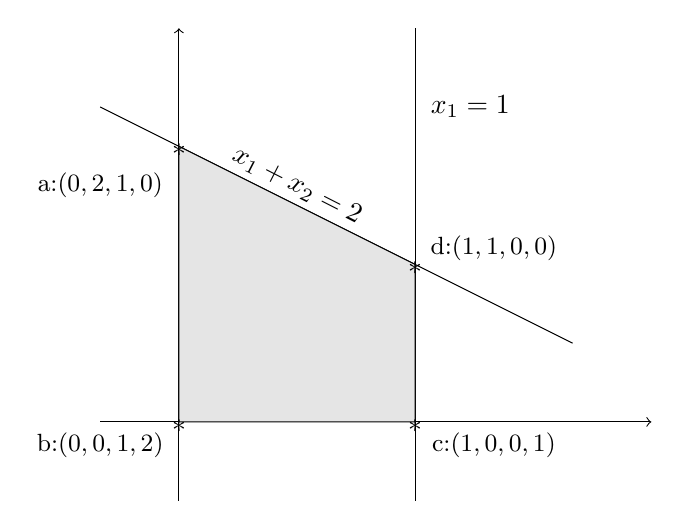
\begin{tikzpicture}
	\draw [->] (5,-1) -- (5,5);
    \draw [->] (4,0) -- (11,0);
	\draw [] (4,4) -- (10,1);
	\draw [] (8,-1) -- (8,5);
	\filldraw[draw=black, fill=gray!20] (5,0) -- (8,0) -- (8,2) -- (5,3.5) -- cycle;
	\node[] at (8.7,4) {$x_1 = 1$};
	\node[rotate=-27] at (6.5,3) {$x_1 + x_2 = 2$};
	\node[] at (8,-0.1) {*};
	\node[] at (8, 1.9) {*};
	\node[] at (5, -0.1) {*};
	\node[] at (5, 3.4) {*};
	\node[] at (4,3) {\small{a:$(0,2,1,0)$}};
	\node[] at (4,-0.3) {\small{b:$(0,0,1,2)$}};
	\node[] at (9,-0.3) {\small{c:$(1,0,0,1)$}};
	\node[] at (9,2.2) {\small{d:$(1,1,0,0)$}};
	\end{tikzpicture}
	\caption{Constraints and vertices of the polytope}
	\label{fig1}
\end{figure}

Let us consider the following linear programming problem as an example, 
\begin{equation*}
\min \text{ } x_1+2x_2, \text{ subject to } x_1 \leq 1 \text{, } x_1 + x_2 \leq 2\text{, } x_1 \geq 0\text{, } x_2 \geq 0
\end{equation*}
Adding slack variables $x_3$ and $x_4 \in S$ to the constraints to convert to standard form, we get
\[
A =  \begin{bmatrix}
1 & 0 & 1 & 0 \\
1 & 1 & 0 & 1
\end{bmatrix}
, b = \begin{bmatrix}
1 \\
2
\end{bmatrix}
, c = \begin{bmatrix}
1 \\
2
\end{bmatrix}
\]

Figure:~\ref{fig1} illustrates the constraints and the four vertices of the feasible polytope formed by these constraints of the above example. It can be observed that exactly 2 out of 4 variables are non-zero (active) since Rank$(A)=2$ and exactly 1 variable changes to active and 1 variable changes to inactive when we move one vertex to any of its neighbouring vertices.

Also, the solution to this problem lies in one of the vertices of the feasible polytope. This means we have to iterate over $n_{C_m}$ possible vertices to find the optimum solution in a brute force approach. This is combinatorically expensive and so simplex method provides an efficient way of searching this set of vertices.

\subsection{Definitions}
\label{def}

\begin{itemize}
	\item $\mathcal{B}$ denotes the subset of index set $\mathcal{I} = \{1,2,\dots,n\}$ containing exactly $m$ indices such that $i \notin \mathcal{B} \implies x_i = 0$. This is called the basic set.
	\item $B = [A_i]_{i \in \mathcal{B}}$ denotes a non-singular $m\times m$ matrix called as the basic matrix.
	\item $\mathcal{N}$ denotes the non-basic set $\mathcal{N} = \{1,2,\dots,n\}\setminus\mathcal{B}$ containing $n-m$ indices such that $i \in \mathcal{N} \implies x_i = 0$.
	\item $N = [A_i]_{i \in \mathcal{N}}$ denotes a $m\times (n-m)$ matrix called as the non-basic matrix.
	\item $x, c \text{ and } S$ are partitioned as basic and non-basic vectors and are defined as below,
	      \begin{center}
				$x_B = [x_i]_{i \in \mathcal{B}}$ ~~~~~~ $x_N = [x_i]_{i \in \mathcal{N}}$ \\
				$c_B = [c_i]_{i \in \mathcal{B}}$ ~~~~~~ $c_N = [c_i]_{i \in \mathcal{N}}$ \\
				$S_B = [S_i]_{i \in \mathcal{B}}$ ~~~~~~ $S_N = [S_i]_{i \in \mathcal{N}}$ \\
	      \end{center}		  
\end{itemize}

\subsection{Mechanics}

The fundamental idea is to move from a feasible vertex to one of its feasible neighbours efficiently and continue to do this till the optimum is reached. In each movement, one index from basic set is swapped with an index from non-basic set. We apply the KKT first order conditions to derive the algorithm. We have
\begin{equation}
Ax = Bx_B + Nx_N = b \text{ and } x_N = 0 \implies x_B = B^{-1}b
\end{equation}
Also we have from KKT conditions,
\begin{equation*}
	A^T\lambda+S = c
\end{equation*}
\begin{equation}
		B^T\lambda+N^T\lambda+S_B+S_N=c_B+c_N
\end{equation}
We choose $S_B = 0$ so as to satisfy complementarity KKT condition $(x^TS=0)$. The above equation is then partitioned as,
\begin{equation*}
B^T\lambda = c_B \text{ and } N^T\lambda+S_N=c_N
\end{equation*}
\begin{equation}
\implies \lambda = (B^T)^{-1}c_B
\label{eqn3}
\end{equation}
\begin{equation}
\implies S_N = c_N - (B^{-1}N)^Tc_B
\end{equation}
$S_N$ is called as the \emph{pricing variable} and its components are called as the \emph{reduced costs} of the non-basic variables $x_N$. They denote the unit decrease in objective function that can be achieved by using the corresponding $x_N$.

A new index $q$ is chosen from $\mathcal{N}$ such that $s_q \in S_N$ is the most negative value. This ensures that the objective decreases by largest possible value. If $s_q \geq 0, \forall q \in \mathcal{N}$, then the optimum is found and algorithm is terminated. Let $x^+$ be the new iterate and we have
\begin{equation*}
Ax^+ = Bx^+_B + A_qx^+_q = Bx_B = Ax
\end{equation*}
\begin{equation}
\implies x^+_B = x_B - B^{-1}A_qx^+_q
\label{eqn5}
\end{equation}
At the new vertex, $x_p = 0, p \in \mathcal{B}$. This index $p$ is removed from $\mathcal{B}$ and moved to non-basic set $\mathcal{N}$. If $p$ is not unique, then we have a degenerate case which is dealt in a different manner not in the scope of this lecture. We will look at how the objective function gets affected by this process. From eqn. \ref{eqn5} we have
\begin{equation}
c^Tx^+ = c^T_Bx^+_B + c_qx^+_q = c^T_Bx_B - c^T_BB^{-1}A_qx^+_q + c_qx^+_q
\label{eqn6}
\end{equation}
From eqn. \ref{eqn3}, $c^T_BB^{-1} = \lambda^T$ and $A^T_q\lambda = c_q - s_q$. Therefore,
\begin{equation*}
c^T_BB^{-1}A_qx^+_q = (c_q - s_q)x^+_q
\end{equation*}
Substituting the above equation in \ref{eqn6}, we get
\begin{equation*}
c^Tx^+ = c^T_Bx_B + c_qx^+_q - (c_q - s_q)x^+_q
\end{equation*}
\begin{equation}
\implies c^Tx^+ = c^Tx + s_qx^+_q
\label{eqn7}
\end{equation}
Since we chose q such that $x_q \le 0$, objective is decreased whenever $x^+_q \ge 0$. If it is possible to increase $x^+_q$ to $\infty$ without encountering a new vertex, then the problem is unbounded.

\subsubsection*{Theorem 1 (13.4 from \cite{nocedal2006numerical})} 
If the linear program is nondegenerate and bounded, the simplex method terminates at a basic optimal point.

\subsection{Algorithm}

\nocite{*}

The overall algorithm for a single iteration is described below. The inputs are $\mathcal{B}$, $\mathcal{N}$, $A$, $b$, $c$ and $x_N=0$ and the outputs are $\mathcal{B^+}$, $\mathcal{N^+}$ and $x^+_B$.

\begin{algorithm}[H]
	\caption{Revised Simplex}
	\begin{algorithmic}[1]		
		\Function{Simplex}{$\mathcal{B},\mathcal{N},A,b,c$}
		\State Obtain $B$ and $N$ as given in section \ref{def}
		\State Solve $Bx_B = b$ for $x_B$.
		\State Solve $B^T\lambda = c_B$ for $\lambda$.
		\State Compute $S_N = c_N - N^T\lambda $.		
		\If {$S_N \geq 0$}
			\State Found Optimal. Terminate algorithm.
		\Else
			\State Select $q \in \mathcal{N}$ where $s_q$ is the most negative.
			\State Solve $Bd = A_q$ for $d$.
			\If {$d \leq 0$}
				\State Unbounded problem. Terminate Algorithm.
			\Else
				\State $x^+_q = \min_{i, d_i \ge 0} \frac{(x_B)_i}{d_i}$. Let $p$ denote the minimizing $i$. \Comment{Ratio Test} 
				\State $x^+_B = x_B - dx^+_q$
				\State $x^+_N = (0,\dots,0,x^+_q,0,\dots,o)^T$
				\State Change $\mathcal{B^+} = (\mathcal{B} \setminus \{p\}) \cup \{q\} $, $\mathcal{N^+} = (\mathcal{N} \setminus \{q\}) \cup \{p\} $
			\EndIf
		\EndIf
		\EndFunction
		
	\end{algorithmic}
\end{algorithm}

It must be noted that the value of objective decreases in most of the steps but not always.

\section{Additional Notes}

There are several challenges and common pitfalls in implementing the revised simplex algorithm. These include pricing and selection of the entering index; starting the simplex method and handling degenerate steps. It is suggested to go through the Section $13.5$ from \cite{nocedal2006numerical} for more details. Also, there are other techniques collectively known as Interior-Point Methods to efficiently solve LP. Details of these can be found in Chapter $14$ of \cite{nocedal2006numerical}.

\printbibliography

\end{document}